\documentclass[conference]{IEEEtran}

\usepackage{url}
\usepackage{multirow}
\usepackage{array}
\usepackage{epsfig}
\usepackage{footnote}
\usepackage{amsmath}
\usepackage{algorithmic}

%\setlength{\parskip}{0pt}
%\setlength{\parsep}{0pt}
%\setlength{\headsep}{0pt}
%\setlength{\topskip}{0pt}
%\setlength{\topmargin}{0pt}
%\setlength{\topsep}{0pt}
%\setlength{\partopsep}{0pt}
%\setlength{\floatsep}{5pt}
%\setlength{\textfloatsep}{5pt}
%\setlength{\intextsep}{5pt}

\widowpenalty=10000
\clubpenalty=10000

\begin{document}

\title{On the Design of  Autonomic, Decentralized VPNs}

\author{
\IEEEauthorblockA{
  David Isaac Wolinsky,
  Kyungyong Lee,
  P. Oscar Boykin,
  Renato Figueiredo
}
\IEEEauthorblockN{
  University of Florida
}
}

\maketitle
\begin{abstract}

Decentralized and P2P (peer-to-peer) VPNs (virtual private networks) are
becoming quite popular to connect users in small to medium collaborative
environments, such as academia, businesses, and homes.  In the realm of VPNs,
there exist centralized, decentralized, and P2P solutions.  Centralized systems
require that at least a single entity providing an infrastructure for everyone,
decentralized approaches allow more than entity to share the responsibility for
this infrastructure, while existing P2P approaches rely on a centralized
infrastructure but allow users to bypass the centralized infrastructure to form
direct low latency, high throughput links.  In this paper, we describe a novel
VPN architecture that can claim to be both decentralized and P2P using methods
that limit the entry barrier for VPN deployment.  Our solution extends existing
work, IPOP (IP over P2P), to address challenges of configuration, management,
and bootstrapping to create cryptographically secure, self-contained P2P
systems.  In doing so, we present the first implementation and analysis of a
P2P system secured by DTLS (datagram transport layer security) along with
decentralized techniques for revoking user access.

\end{abstract}

\section{Introduction}

A Virtual Private Network (VPN) provides the illusion of a local area network
(LAN) spanning a wide area network (WAN) by creating secure\footnote{For the
remainder of this paper, unless explicitly stated otherwise, security implies
encryption and mutual authentication between peers.} communication links
amongst participants.  Common uses of VPNs include secure access to enterprise
network resources from remote/insecure locations, connecting distributed
resources from multiple sites, and establishing virtual LANs for multiplayer
video games and media sharing over the Internet.

The architecture described in this paper addresses usage scenarios where VPNs
are desired but complexity in deployment and management limits their
applicability.  Such as collaborative academic environments linking individuals
spanning multiple institutions, where coordinated configuration of network
infrastructure across the different sites is often impractical.  Another
example is the small/medium business (SMB) environment, where it is often
desirable to securely connect desktops and servers across distributed sites
without incurring the complexity or management costs of traditional VPNs.  Such
a VPN could be used to enable extended families to share media, such as family
videos and pictures, with each other, where existing VPNs may be too
complicated or the hosting a centralized service may be undesirable.

Explicitly, the model considered in this paper is motivated from our
Archer~\cite{archer} project.  Archer provides a dynamic and decentralized grid
environment for computer architecture researchers to share and access voluntary
compute cycles with each other.  Use of centralized systems would limit the
scope of Archer and require dedicated administration from multiple parties,
whereas decentralized solutions require manual configuration of links between
peers, which is beyond the scope of the target users.  Current P2P VPN
approaches either lack scalability or proper security components to be useful
for VPN approaches.

We began our original foray into user-friendly VPN approaches with
IPOP~\cite{ipop}.  Previous work on IPOP focused on the routing mechanisms and
address allocation with multiple virtual networks (VNs) sharing a single P2P
overlay.  Deploying a private overlay would require the user to deploy their
own infrastructure including necessary security underlay, such as IPsec, at
which point, at which point a P2P VPN becomes irrelevant.  Sharing an overlay
has significant drawbacks.  A misconfigured peer could easily disable the
entire overlay, rendering all VPNs useless, and the system would have to be
recreated as there exists no methods to remove the peer from such a system.
Without a shared overlay, each VPN would need to deploy a P2P infrastructure
prior to the VPN system, at which point, users may reconsider the approach and
prefer a more traditional centralized approach.

To make an easy-to-use, fully decentralized and P2P VPN, we extend the IPOP
concept to support bootstrapping from public infrastructures and overlays into
private P2P overlays whose membership is limited to an individual VPN user
base.  The key concept behind our work is based upon Castro et
al.~\cite{one_ring}, who suggests a single overlay for bootstrapping service
overlays.  A private overlay by itself is secured only by obfuscation,
malicious peers may eventually discover, join, and violate the overlay.  As
such, we present the first implementation and evaluation of an overlay with
secure communication between end points in the P2P overlay and communication
inside the P2P overlay.  Security without revocation for misbehaving peers can
ultimately lead to corrupted overlays but current revocation techniques rely on
centralized systems, we present means to revoke using the P2P overlay itself.
We call the completed system and the interface used to administrate it
GroupVPN, a novel VPN architecture that extends IPOP to create a novel secured
decentralized P2P VPN.

The rest of this paper is organized as follows.  Section~\ref{background}
describes the current IPOP architecture.  Current IPOP systems lack security,
we present a framework for securing both IPOP and the P2P overlay in
Section~\ref{security}.  Section~\ref{revocation} overviews our approaches for
decentralized certificate revocation.  The complete system, GroupVPN, is
presented in Section~\ref{groupvpn}.  Section~\ref{related_work} compares and
contrasts our work with related work.  Section~\ref{conclusions} concludes the
paper.

\section{Background}
\label{background}

This section describes the basic construction of IPOP, a structured P2P virtual
network including background on structured overlays, address allocation and
discovery, and connectivity.

\subsection{P2P Overlays}

The type of P2P overlay chosen for a VPN will have an effect on how easy the
VPN is to program, deploy, secure, how efficient it is, and how it will deal
with growth.  The two primary infrastructures for P2P overlays are unstructured
and structured systems.  Unstructured systems use mechanisms such as global
knowledge, broadcasts, or stochastic techniques~\cite{unstruct_v_struct} to
search the overlay, as the system grows, maintaining this state and searching
for things requires complex algorithms and mechanisms to retain efficiency.
Alternatively, structured approaches maintain provide guaranteed search times
typically with a lower bound of $O(\log N)$ regardless of network size.  In
terms of complexity, for small systems, unstructured systems may be easier to
implement but as the system grows it may become inefficient.

IPOP uses a structured P2P framework named Brunet~\cite{brunet}, which is based
upon Symphony~\cite{symphony}.  Structured systems are able to make guarantees
about efficiencies by self-organizing into well-defined topologies, such as a 1
dimensional ring or a hypercube, each member having a unique identifier, a P2P
address.  Links in the overlay are made to guarantee the efficient search time.
In addition, Brunet automatically creates links between heavily trafficked
peers for efficiency in IPOP.

A key component of most structured overlays is support for decentralized
storage/retrieval of information called a distributed hash table (DHT).  The
DHt builds upon the existence of a P2P address space.  All peers in a
structured system have a unique, uniformly distributed P2P address.  A DHT maps
look up values or keys usually by a a hashing function into the P2P address
space.  While there are various forms of fault tolerance, a minimalist DHT
stores values at the node whose address is closest to the value's key.  DHTs
can be used coordinate organization and discovery of resources, making them
attractive for self-configuration and organization in decentralized
collaborative environments.  As explained in the next section, IPOP, uses a DHT
to coordinate decentralized organization.

\begin{figure*}[ht]
\centering
\includegraphics[width=3in,angle=-90]{figs/bootstrap_brunet_light.ps}
\caption{Bootstrapping a private overlay using Brunet}
\label{fig:bootstrap}
\end{figure*}

\subsection{Connecting to the VPN}

To connect to IPOP, a peer need only connect to an existing Brunet
infrastructure.  Many IPOP systems can coexist sharing a single overlay.  The
motivation for doing so is that bootstrapping a P2P system can be challenging,
requiring users to understand concepts such as IP addresses and ports, as well
as having access to a public IP address or being able to configure a router or
firewall to enable inbound connections.

A peer connected to IPOP's P2P infrastructure can take advantage of its support
for NAT traversal through hole punching~\cite{ice}.  When performing hole
punching, peers first obtain mappings of their private IP address and port to
their public IP address and port and then exchange them over a shared medium,
in this case the P2P overlay.  The peers attempt to simultaneously form
connections with each other, tricking NATs and firewalls into allowing inbound
connections, because the NAT believed an outbound flow already exists.  In case
peers cannot establish direct connectivity, messages can be relayed through the
P2P overlay to each other though with added latency and limited throughput.

This approach not only enables peers behind NATs and firewalls to seamlessly
connect to each other, without requiring peers to host their own bootstrap
servers.  If a peer were to host their own bootstrap servers, they first need a
public IP address and bind the application to a port on that system.  At which
point, they could share the IP, port pair with other peers in the VPN.  Though
if they were to go offline or their IP address were to change the P2P
infrastructure, new users would be unable to join.

\subsection{Organization}

In the context of VPNs, structured overlays can handle organization of the
network space, address allocation and discovery, decentrally through the use of
a DHT, such systems have been proposed in~\cite{pcgrid07,i3}.  Membership in
the VPN includes a matching membership in the structured overlay, thus all VPN
peers have a P2P address.  To address the challenges of having multiple VPNs in
the same overlay, each IPOP group has its own namespace, reducing the
likelihood of overlap.  To enable scalable and decentralized address allocation
and discovery, peers store mappings of IP address to P2P address into the DHT,
typically of the form $hash(namespace + IP) = P2P address$.  Thus a peer
attempting to allocate an address will insert this key, value pair into the
overlay.  The first peer to do this will be the owner of the IP address
allocation.  Therefore the DHT must support atomic writes into the DHT.

Mechanisms to self-configure the IP address and network parameters of the local
system can be provided by DHCP (decentralized host configuration protocol),
manually configuring the IP address, or the VPN hooking into OS APIs.  Address
discovery is initiated when an outgoing packet for a remote peer arrives at the
VPN software.  At which point, the VPN will query the DHT with the IP address
to obtain the owner's P2P address and forward the packet to the destination.
Discussion on both these topics is further covered in our previous
work~\cite{sc09}.

\section{Evaluation Tools}

As mentioned earlier, IPOP uses Brunet as the underlying P2P infrastructure for
connectivity.  Brunet has been in active development for the past 5 years.
Prior to releasing updates, the code is run on PlanetLab~\cite{planetlab} for a
period of 2 weeks.  PlanetLab consists of of nearly 1,000 resources distributed
across Earth.  In practical application, though, roughly 40\% of the resources
are unavailable at any given time and the remaining behave somewhat
unpredictably.  This unpredictability provides behavior, that many times, is
far more effective at finding bugs than users tests.

Deploying on PlanetLab takes approximately 15 minutes to bootstrap all the
resources and then many more to verify a certain behavior, making regression
testing and verification tests complicated.  To address this, we have extended
Brunet to support a simulation mode, where time is based upon a virtual timer
incremented based upon an event driven scheduler.  Furthermore, the simulation
framework also uses a specialized transports layer to avoid the overhead of
using TCP or UDP on the host system, both of which are limited resources and
can hamper the ability to simulate large systems.  In addition, they offer few
if any additional insights into system performance.  The specialized framework
uses datagrams to pass messages between nodes, thus from the nodes perspective,
it is very similar to a UDP transport and can simulate both latency and packet
dropping.  In this paper, we set the latency between all node pairs to 100 ms.

Both simulation and real system evaluation provide unique advantages.
Simulations allow faster than real time execution of reasonable sized networks
(up to a few thousand) using a single resource, while enabling easy debugging.
Where as deployment on real systems presents opportunities to add more chaos
into the system which can be difficult to duplicate in simulation, such as
occassional network glitches, CPU delays on processing, and other random
difficult to ascertain events.

For the purpose of this paper, we will perform experiments using both deployed
systems either on local resources and PlanetLab or using simulation.  The
various evaluations dictate, which mechanism we use.  Though when possible, we
evaluate with as many as possible, thus verifying the system.

\section{Towards Private Overlays}

Many users of IPOP began by trying the shared overlay and, once comfortable,
attempt to host their own infrastructure.  Some are successful without
assistance from us, while a majority are not.  The most common issue preventing
users from hosting their own independent IPOP systems was the result of network
configuration issues.  In short, users were able to easily join the shared
overlay, but similar attempts to construct their own were hindered.

The motivation for a private IPOP overlay is quite clear, a shared overlay
provides no means for controlling access and can easily be tampered.  Though
bootstrapping a P2P system requires expertise in network administration.  To
enable users to bootstrap their own private overlays, we previously
investigated means by which a public overlay could be used to bootstrap a
private overlay.

Our approach for bootstrapping private systems requires an overlay to support a
methods for peers to discover each other, relay messages, and obtain their
public address mapping as described in our recent paper~\cite{p2p10}, that
focuses on bootstrapping P2P systems.  Examples of other potential bootstrap
overlays include popular and well established P2P systems, such as Gnutella,
Skype, and Kademlia.  Our initial work supports bootstrapping from XMPP
(Jabber) systems and our own P2P overlay, Brunet.

To bootstrap from an existing Brunet overlay, peers first insert their public
overlay address into the key represented by $hash(\$Private Overlay Namespace)$
and continue to do so regularly until they disconnect, so as to not let the
entry become stale and disappear.  Peers attempting to bootstrap into the
private overlay can then query this key and obtain a list of public overlay
nodes that are currently acting as proxies into the private overlay.  By using
the public overlay as a transport, similar to UDP or TCP, the private overlay
node forms bootstrapping connections via the public overlay.  At which point,
overlay bootstrapping proceeds as normal.  The entire process is represented in
Figure~\ref{fig:bootstrap}.

In a small private overlay, there is a reasonable chance that not a single node
in that overlay has a public address, making it difficult for the overlay to
provide its own form of NAT traversal services.  Rather than having a special
case for NAT traversal for the private overlays that differentiates from the
public overlay it bootstrapped from, the two share underlying TCP and UDP
sockets.  This mechanisms, known as pathing, allows a single UDP socket and
listening TCP socket to create links for many overlays.  This is only possible
due to the generic transports library, which does not differentiate UDP, TCP,
or even relayed links.  Thus during link establishment, the pathing system acts
as a proxy, by intercepting a link creation request from a specific entity,
mapping that to a path, and then requesting from the remote entity a link for
that path.  The underlying link is then wrapped by pathing and given to the
correct overlay node.  Resulting in a completely transparent multiplexing of a
TCP and UDP socket enabling the NAT traversal in one overlay to benefit the
other.  Furthermore, once a link has been established, the pathing information
is irrelevant, limiting the overhead into the system to a single round trip
time in the bootstrapping phase.

\subsection{Time to Bootstrap a Private Overlay}

In our previous work~\cite{p2p10}, we only verified that private overlays could
be bootstrapped using a small set of resources, 5, behind NATs.  The focus of
this paper extends beyond that paper and emphasizes overheads.  This evaluation
uses both PlanetLab and simulation to determine the delay in bootstrapping an
IPOP-only overlay from a public shared overlay in constrast to a common IPOP
overlay.  100 tests were run for each of the various network sizes.  In the
case of simulation, a new network was generated for each test, while PlanetLab
reused the same overlay, but the joining peer changed its P2P address as to
cause the peer to connect to a different set of nodes in the public overlay.
The results are presented in Figure~\ref{fig:private_bootstrapping}.

\begin{figure}[ht]
\centering
\includegraphics[width=3in]{figs/bootstrap.eps}
\caption{}
\label{fig:private_bootstrapping}
\end{figure}

There are two important details that we would like to share.  First, the
PlanetLab side of the experiment is extremely limited in the smaller sized
networks, as the system stayed static and a poorly connected peer can shift the
results significantly.  We have only included the results to show that the
techniques do scale for large systems.  Second, simulation of the
bootstrapping, we discovered that use the simplistic algorithm describe earlier
sometimes would result in partitioned overlays.  The cause was due to peers
determining from a random subset of the peers they initiated connections with
that they were connected to the complete overlay, but in reality, they were
forming partitions.  Because the peers thought they were fully connected, the
overlays would never fix the partitioning.  To address this, we have set it so
that peers occassionally query the DHT entry to determine if there is a peer in
the list that should be directly connected to them but is not.  If such a peer
exists, the searching peer begins connection procedures with that peer.

\subsection{Overhead of Pathing}

Much like the previous experiment, this one too is used to verify the use of
the private overlay bootstrapping components for VPN usage.  In this case, the
pathing technique is evaluated to determine what overheads may exist by using
the approach.  To determine the overheads, two IPOP VNs are deployed on
resources on the same gigabit LAN using netperf to evaluate both latency and
throughput.  We ignore the other specifications of the machines as we compare
both the system with pathing versus the system without pathing.  The results
are presented in Table~\ref{tab:pathing}.  The results indicate that the use of
pathing presents negligible overhead for both throughput and latency, making it
a very worthy trade to transparently deal with NAT and firewall traversal.

\begin{table}[ht]
\centering
\begin{tabular}{|c||c|c|}
\hline & Latency (ms) & Throughput (Mbit/s) \\ \hline \hline
Standard & 0 & 0 \\ \hline
Pathing & 0 & 0 \\ \hline
\end{tabular}
\caption{Pathing overheads}
\label{tab:pathing}
\end{table}

\section{Security for the Overlay and the VPN}
\label{security}

Structured overlays are difficult to secure and a private overlay does not
imply that it is safe from malicious users as it provides no means to limit
access to the system.  Malicious users can pollute the DHT, send bogus
messages, and even prevent the overlay from functioning, rendering the VPN
useless.  To address this in means that make sense for VPNs and common users,
we have employed a public key infrastructure (PKI) to encrypt and authenticate
both communication between peers as well as communication between peers through
the overlay, called point-to-point (PtP) and end-to-end (EtE) communication,
respectively.

The motivation for using a PKI is that users can either pre-exchange public
keys through a trusted medium or place their trust into a third party known as
a certificate authority (CA).  Unlike other security systems, in particular a
key distribution center, which relies on a middleman to establish secure
sessions, a CA system enables two peers who have previously obtained a CA
signed certificate to establish a trusted relationship directly.  So not only
can peers form a relationship directly, they can do so without requiring that
the CA be online.

The reasons for securing PtP and EtE are differnt.  Securing PtP communication
prevents unauthorized access to the overlay, as peers must authenticate with
each other for every link created.  Though once authenticated, a peer can
perform malicious acts and since the overlay allows for routing over it, the
peer can disguise the origination of the malicious acts.  By also employing EtE
security, the authenticity of messages transferred through an overlay can be
easily verified.  Though EtE security by itself, will not prevent unauthorized
access into the overlay.  By employing both PtP and EtE, overlays can be
secured from uninvited guests from the outside and can easily identify
malicious users on the inside.  Implementing both leads to important questions:
what mechanisms can be used to implement both and what are the effects of both
on an overlay and to a VPN on an overlay.

\subsection{Implementing Overlay Security}

There are various types of PtP links, for example, there are TCP and UDP
sockets, relays across nodes and overlays, and explored in previous work relays
across external services like XMPP.  EtE communication is strictly datagram
unless the overlay employs a userspace stream based relability service.
Traditional approaches of securing communication such as IPsec or SSL will not
apply, nor will approaches that rely on reliable, in order connections such as
SSL or TLS.  As such, we have implemented an abstraction akin to a security
filter as presented in Figure~\ref{fig:security_filter}, which enables the use
of security libraries and protocols that are not reliant on strict interfaces.
To this date, we have implemented both a DTLS~\cite{dtls} filter using the
OpenSSL implementation of DTLS as well as a protocol that reuses cryptographic
libraries provided by .NET that behaves similarly to IPsec.

A security filter has two components, the manager and individual sessions or
filters.  While the individual sessions could act as filters by themselves, by
combining with a manager, they can be configured for a common purpose and
security credentials.  This approach enables the use of security to be
transparent to the other components of the system as the manager handles
session establishment, garbage collection of expired sessions, and revocation
of peers.

\begin{figure}[ht]
\centering
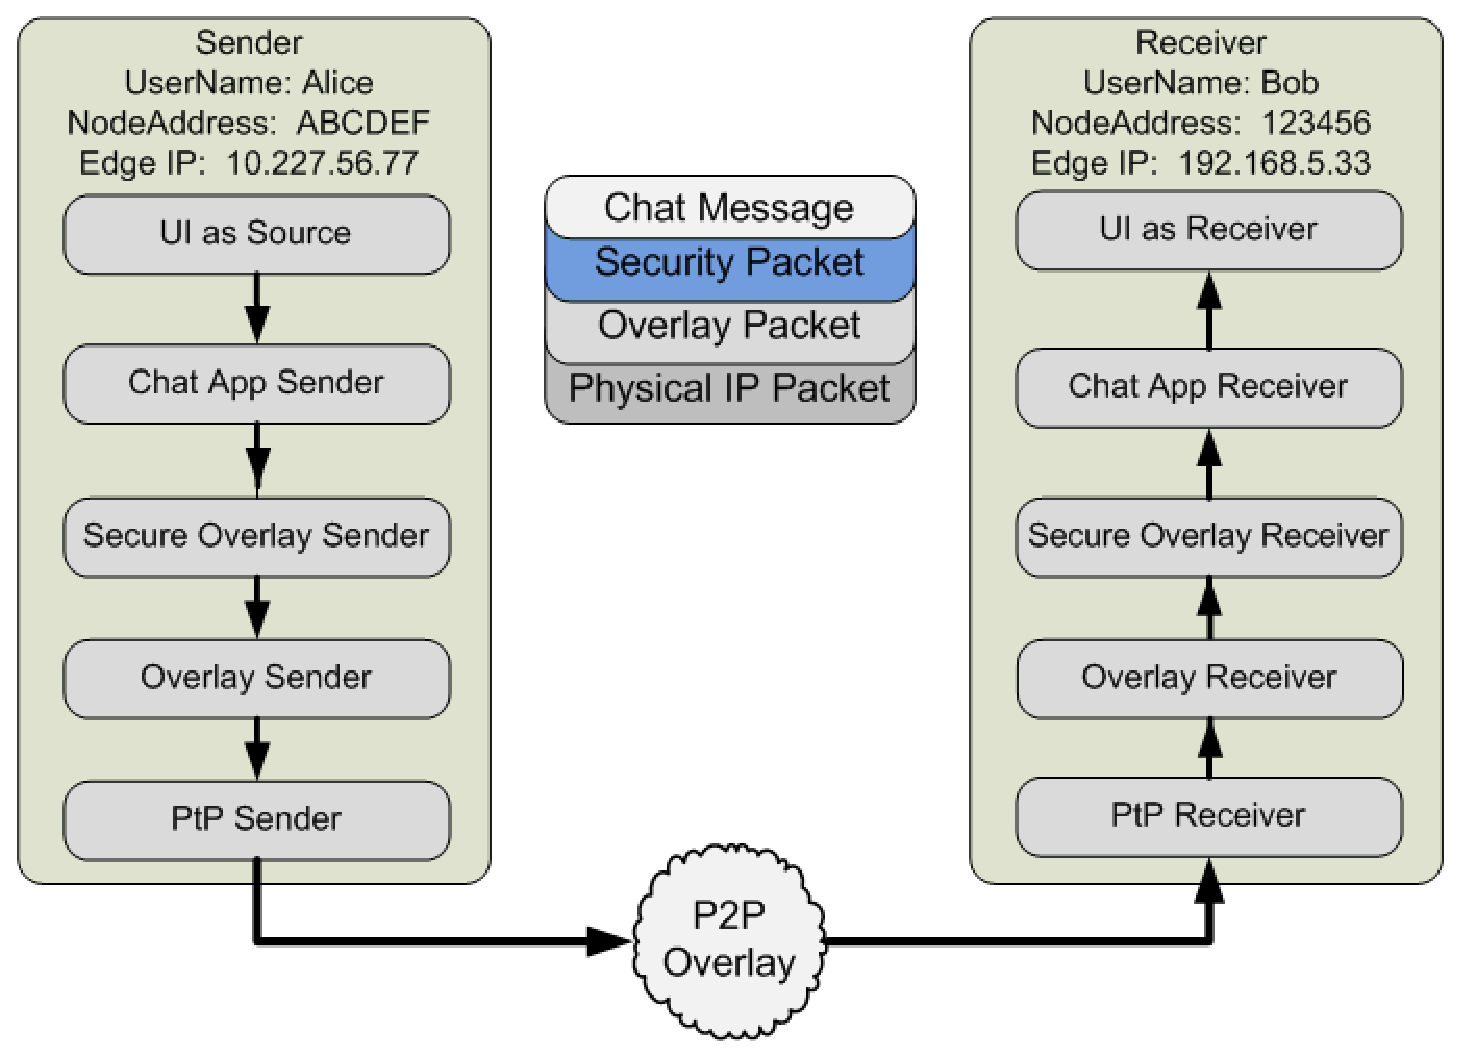
\includegraphics[width=3.25in]{figs/secure_sender_stack_generic.png.eps}
\caption{An example of the abstraction of senders and receivers using a EtE 
secured chat application.  Each receiver and sender use the same abstracted
model and thus the chat application requires only high-level changes, such
as verifying the certificate used is Alice's and Bob's, to support security.}
\label{fig:security_filter}
\end{figure}

The strength in using certificates is the embedding of identity in the
certificate.  In network systems, the certificate uses the domain name to
uniquely identify and limit the use of a certificate.  When a CA signs the
certificate, by including the domain name, it ensures that users can almost
blindly trust that a certificate is valid, while used to secure traffic to that
domain.  Communication with another domain using the same certificate will
raise a flag and will result in the user not trusting the certificate.  In
environments with NATs, dynamic IP addresses, or portable devices, typical of
P2P systems, assigning a certificate to a domain name will be a hassle as it
contrains mobility and the type of users in the system, furthermore, most users
are unaware of their IP address and changes to it.  Instead, a certificate are
signed against the users P2P address.  During the formation of PtP links or
while parsing EtE messages, the two nodes discover each others P2P addresses,
if the addresses do not match the address on the verified certificate, the
communication need not proceed further.  

The use of a filter approach, this requires one change to the core software,
such that it verifies the identity of the remote side prior to allowing packets
to traverse the session.  In our system, we did this by means of a callback,
which presents the underlying sending mechanism, EtE or PtP, and the overlay
address stored in the certificate.  The receiver of the callback can attempt to
cast it into known objects, if successul, it will compare the overlay address
with the sender type.  If unsuccessful, it ignores the request.  If any
callbacks return that the sender does not match the identifier, the session is
immediatley closed.

The last consideration comes in the case of EtE communication that provides an
abstraction layer.  For example, in the case of VPNs, where where a P2P packet
contains an IP packet and thus a P2P address maps to a VPN IP address, a
malicious peer may establish a trusted link, but then hijack another users IP
session.  As such, the application must verify that the IP address in the IP
packet matches the P2P address of the sender of the P2P packet.

\subsection{Overheads of Overlay Security}

When applying an additional layer to a P2P system, there will be obvious
overheads in terms of time to become connected to the overlay.  Other less
obvious effects will be throughput, latency, and processing overheads, this is
primarily due to the use of the P2P system over a wide area network, where the
latency and throughput limitations due to the network conditions between two
points will make the overhead of security negligible except in the case of
bootstrapping due to additional round trip messages used for forming a secure
connection.

\begin{figure}[ht]
\centering
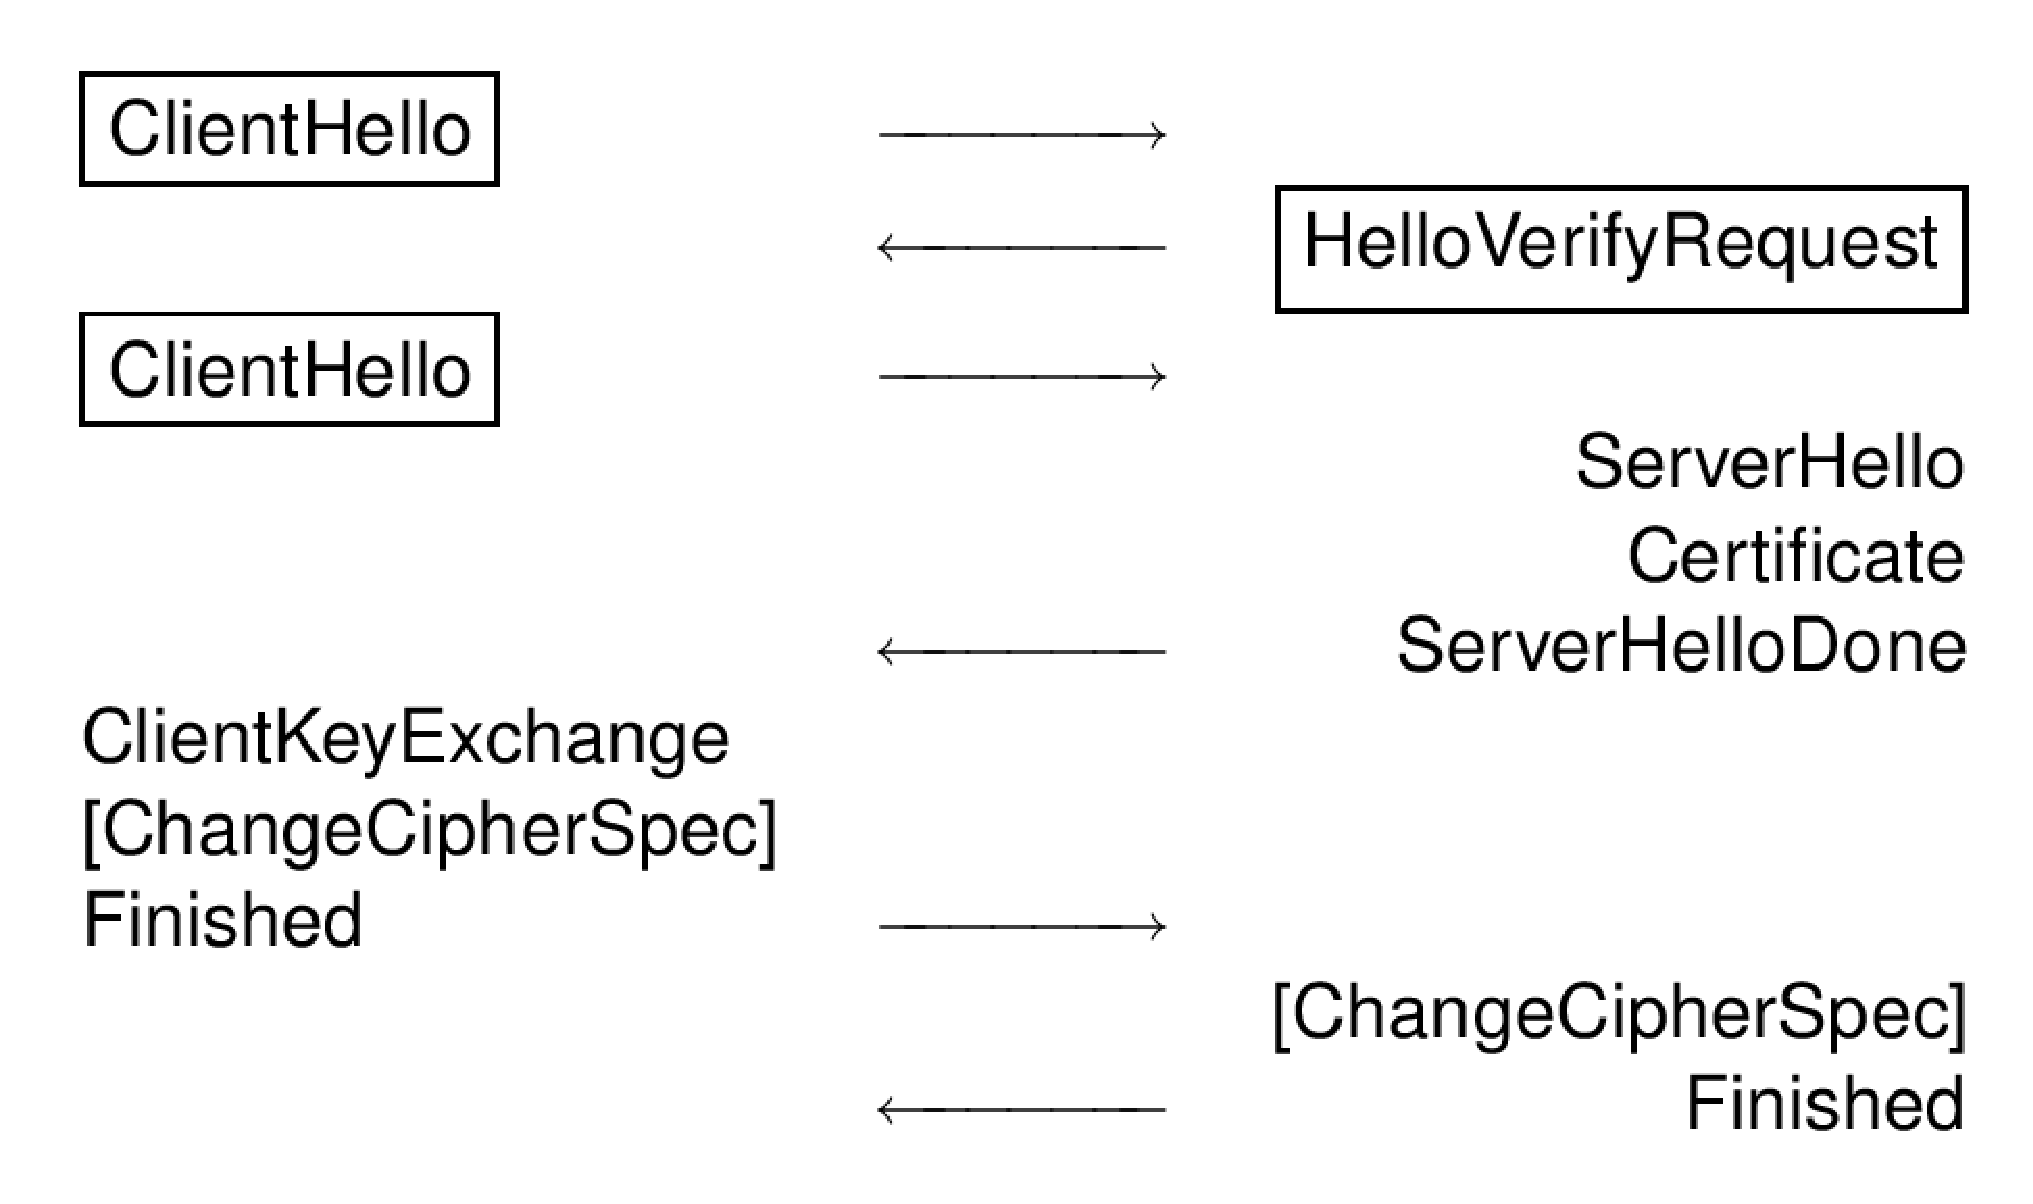
\includegraphics[width=2.5in]{figs/dtls.eps}
\caption{DTLS handshake}
\label{fig:dtls}
\end{figure}

For example, consider the DTLS handshake as presented in Figure~\ref{fig:dtls},
which consists of 6 messages or 3 round trips.  PtP security  may very well
have an effect on the duration of overlay bootstrapping.  There even exists a
possibility that with more messages during bootstrap, the probability one drops
is higher, which could have also, in turn, have an effect, though possibly
negligible, on time to connect.  To evaluate these concerns, we have employed
both simulation and real system experiments.

The following experiments use both the simulation to evaluate time to connect a
new node to an existing resource.  Then another experiment is performed to
evaluate how long it takes to bootstrap various sized overlays if all nodes
join at the same time.  This experiment is only feasible via simulation as
attempting to reproduce in a real system is extremely difficult due how quickly
the operations complete.

\subsubsection{Adding a Single Node}

This experiment determines how long it takes a single node to join an existing
overlay with and without DTLS security.  The experiment is performed using both
simulation and a real deployed system.  After deploying a set of nodes without
security and with security on PlanetLab, a crawl was run to determine the size
of the network.  In both cases, the overlay maintained an average size of
around 600 nodes.  At which point, a new node connected to the overlay 1,000
times, generating a new P2P address each time, and thus connecting to a
different point in the overlay.  As soon as the node believed it had connected
to the correct location in the overlay, the experiment ended.  For simulation
purposes, a new overlay was deployed each time, 100 times, each time a new node
would join.  The test completed after the entire overlay agreed upon being
properly correct, a more rigorous test than that tested in the real system.
The CDF for the experiments is presented in Figure~\ref{fig:add_one}.

\begin{figure}[ht]
\centering
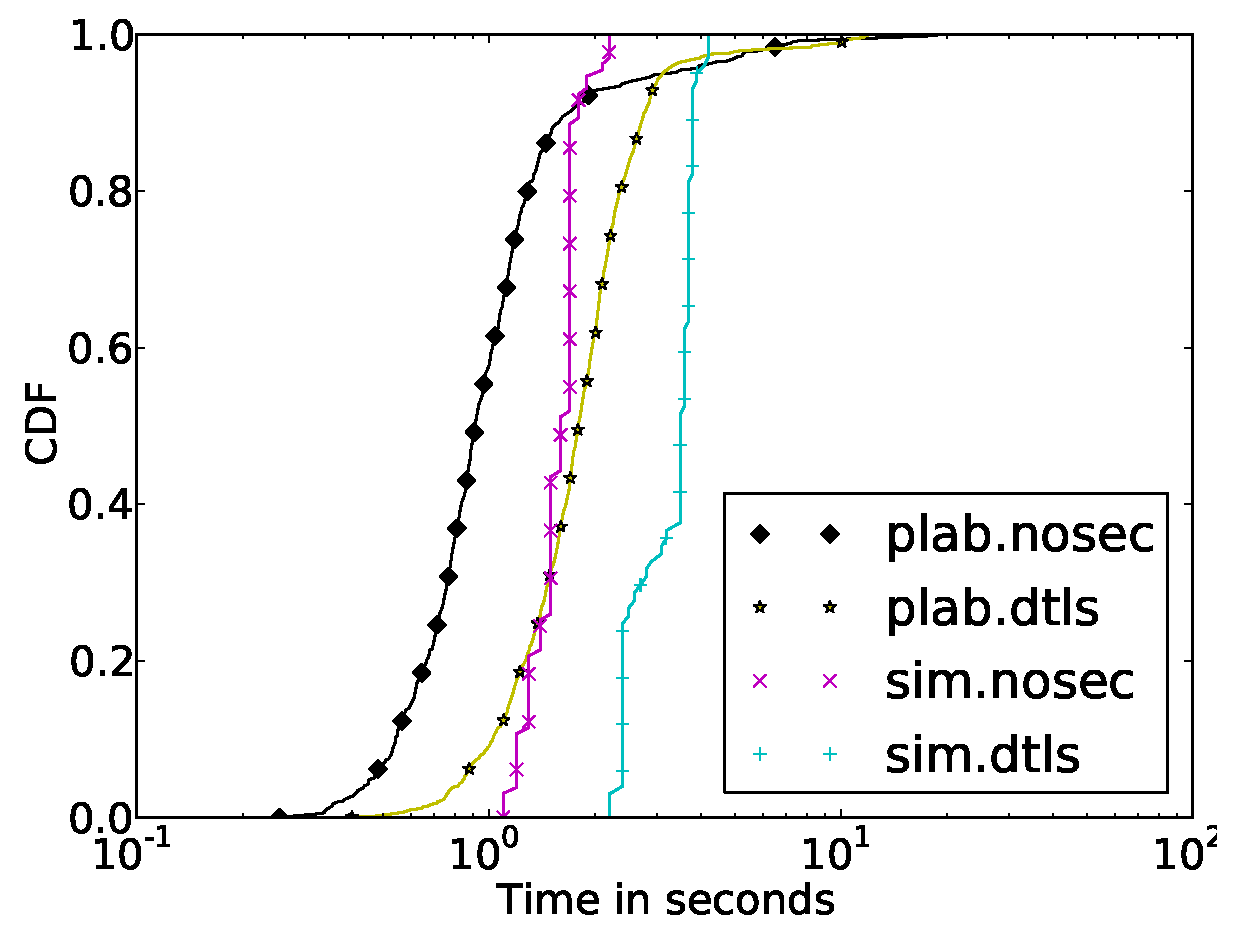
\includegraphics[width=3.5in]{figs/addone.eps}
\caption{Time in seconds for a single node to join a secure (dtls) and insecure
(nosec) structured overlay, using both PlanetLab (plab) and the Simulator
(sim).}
\label{fig:add_one}
\end{figure}

\subsubsection{Bootstrapping an Overlay}

The purpose of this experiment is to determine how quickly an overlay using
DTLS can bootstrap in comparision to one that does not given that there are no
existing participants.  Nodes in this evaluation are randomly given information
about 5 different nodes in the overlay and then all attempt to connect with
each other at the same time.  The evaluation completes after the entire overlay
has all nodes connected and in their proper position.  For each network size,
the test is performed 100 times and the average result is presented in
Figure~\ref{fig:bootstrap_eval}.

\begin{figure}[ht]
\centering
\includegraphics[width=3.5in]{figs/bootstrap.eps}
\caption{Time in seconds for a secure (dtls) and insecure (nosec) structured
overlay to bootstrap, given that all nodes bootstrap simulataneously.}
\label{fig:bootstrap_eval}
\end{figure}

\subsection{Discussion}

Both evaluations show that the overhead in using security is practically
negligible, when an overlay is small.  In the case of adding a single node, it
is clear that the simulation and deployment results agree, as the difference
between bootstrapping into an overlay with and without security remains nearly
the same.  Clearly this motivates the use of security if time to connect is the
most pressing question.

While staring at the graphs, we were quite surprised by how little the time to
bootstrap a secure overlay was than an insecure overlay.  What we realized is
that complex connection handshaking, as implemented in Brunet, can easily
dominate connection time.  For example, in Brunet, two peers must communicate
via the overlay prior to forming a connection, and the system differentiates
between bootstrapping connections and overlay connections.  Thus even though a
peer may have a bootstrapping connection, it will need to go through the entire
process to form an overlay connection with a peer.  The decision for this
process was to keep the code simple and easier to maintain.

\section{Handling User Revocation in a Secure Overlay}
\label{revocation}

Unlike decentralized systems that use shared secrets, in which the creator of
the overlay becomes powerless to control malicious users, a PKI enables the
creator to effectively remove malicious users.  Typical PKIs either use a
certificate revocation list (CRL) or online certificate verification protocols
such as Online Certificate Status Protocol (OCSP).  These approaches are
orthogonal to decentralized systems as they require a dedicated service
provider in order to verify a certificate, if the service provider is offline,
an application can only rely on historical information to make a decision on
whether or not to trust a link.  In a decentralized system, these features can
be enhanced so not to rely on a single provider.  In this section, we present
two mechanisms of doing so: storing revocations in the DHT and performing
overlay broadcast based revocations.

\subsection{DHT Revocation}

A DHT can be used to provide revocation similar to that of OCSP or CRLs, where
users can either query a service provider to obtain the validity of one or more
certificates.  A revocation can be stored in the DHT by signing the hash of a
certificate and the time stamp of revocation and storing all three in the DHT
at the key formed by the hashing of the certificate.  In doing so, revocations
will be uniformly distributed across the overlay, not relying on any single
entity.

The problem with the DHT approach is that it does not provide an event
notification for members currently communicating with the peer.  While peers
could continue to poll the DHT to determine a revocation, doing so is
inefficient.  Furthermore, a malicious peer, who has a valid but revoked
certificate could force every member in the overlay to query the DHT,
negatively affecting the DHT nodes storing the revocation.

\subsection{Broadcast Revocation}

Broadcast revocation can be used to address the deficiencies of DHT revocation.
As a topic of previous research works~\cite{broadcast, chord_broadcast},
structured overlays can be used without additional state to perform efficient
broadcasts from any point in the overlay to the entire overlay.  The form of
broadcast can be used to perform to notify the entire overlay immediately about
a new revocation.  In these papers, analysis and simulations have shown that
the approach can be completed in $O(\log^2 n)$ time.

\begin{figure}[ht]
\centering
\includegraphics[width=2.5in]{figs/tree.eps}
\caption{Broadcast performing a complete overlay broadcast}
\label{fig:tree}
\end{figure}

Our modified algorithm as illustrated in Figure~\ref{fig:tree} utilizes the
organization of a structured system with a circular address space that requires
peers be connected to those whose node addresses are the closest to their own,
features typical of 1-d structured overlays including Chord~\cite{chord},
Pastry~\cite{pastry}, and Symphony.  Using such an organization, it is possible
to do perform a broadcast with no additional state.  To perform a broadcast,
each node performs the following recursive algorithm:
\begin{algorithmic}
\STATE {\bf BROADCAST(start, end, message)}:
  \STATE RECEIVE(message)
  \FOR{$i$ in length(connections)}
    \STATE n\_start $\gets$ ADDRESS(connections$[i]$)
    \IF {n\_start $\not\in$ $[$start, end$)$}
      \STATE continue
    \ENDIF
    \STATE n\_end $\gets$ ADDRESS(connections$[i+1]$)
    \IF {n\_end $\not\in$ $[$start, end$)$}
      \STATE n\_end $\gets$ end
    \ENDIF
    \STATE msg $\gets$ (BROADCAST, n\_start, n\_end, message)
    \STATE SEND(connections$[i]$, msg)
  \ENDFOR
\end{algorithmic}
with ``connections'' as a circular list of connections in non-decreasing order
from the perspective of the node performing the current recursive, broadcast
step.

In this algorithm, broadcast initiator uses its own address as the start and
end, thus the broadcast will span the entire overlay after completing recursive
calls at each connected node.  A recursive end, ``n\_end'', must be inside the
region between ``start'' and ``end'', thus if the connection following the
current sending connection, ``connections$[i+1]$'', is not in that region, it
will only broadcast up to ``end'' and not the address specified by that
connection.  Finally, nodes, who have a connection to the malicious peer, will
end the connection prior to accidentally forwarding the message to the peer by
receiving and acting upon the revocation prior to forwarding the message.  To
summarize, the overlay is recursively partitioned amongst the nodes at each hop
in the broadcast.  By doing so, all nodes receive the broadcast without
receiving duplicate broadcast messages.

\subsection{Evaluation of Revocation Models}

%Figure~\ref{fig:revocation} presents the time required to perform a revocation
%using the simulator described in Section~\ref{security.evaluation}.  After the
%system establishes steady state, a random node is selected to be revoked.  This
%evaluation measures the time to perform such a revocation.  In the case of a
%broadcast a broadcast revocation, this is the time for a message to be
%distributed to the entire overlay, whereas in the case of DHT, it is the time
%to perform the DHT insertion.

%The results seem to indicate that in terms of time, network size and bandwidth
%scale well together.  In contrast, the network traffic scales significantly
%better in DHT experiments, though the approach can be inefficient for
%environments consisting of malicious and colluding peers.  In a DHT revocation,
%revoked peers can attempt to connect with new peers who do not know about the
%revocation, causing each of them to query the DHT to discover the revocation.
%If this becomes the case, the DHT method will quickly become inefficient.  On
%the other hand, the broadcast cannot ensure that all nodes receive the message,
%due to overlay network stability issues, peers may not be included in the
%broadcast.  As such the best approach may be to store a revocation in the DHT
%but notify all peers of a revocation via a broadcast.  Broadcast is efficient
%with bandwidth both for the broadcasting peer and the overlay.  The
%broadcasting peer only sends out as many packets as connections it has, while
%the tree formed by broadcast spans exactly N-1 connections.  In other words,
%the network traffic required to do a broadcast on this tree is the minimum
%amount of communication necessary to reach all nodes in the broadcast range.

\begin{figure*}[ht]
\centering
\includegraphics[width=3in,angle=-90]{figs/groupvpn.ps}
\caption{Process in bootstrapping a new GroupVPN instance.}
\label{fig:groupvpn}
\end{figure*}

\subsection{Discussion}

In contrast to the DHT solution, broadcast revocation occurs only once and does
not leave state behind.  Thus the broadcast is not a complete solution, new
peers to the overlay or those who missed the broadcast message will be unaware
of a revocation.  Furthermore, if an overlay is shared by many VPNs, it may
prevent overlay broadcasting or itself may be inefficient.  

The DHT solution by itself may also not sufficient as revocations may be lost
over time as the entries must have their leases renewed in the DHT.  To address
this condition, each peer maintains a local CRL and the owner of the overlay
can occasionally send updates to the CRL through an out of band medium, such as
e-mail.  A better long term solution may be the use of a gossip protocol so
that peers can share their lists with each other during bootstrapping phases.

A key assumption in using these is that a Sybil~\cite{sybil}, or collusion
attack, is difficult in the secured overlay.	 If a Sybil attack is successful,
both a DHT and broadcast revocation may be unsuccessful, though peers could fix
this problem by obtaining the CRL out of band.  In addition, previous
work~\cite{secure_routing} has described decentralized techniques to limit the
probability of such attacks from occurring.  In our approach, the use of
central authority to review certificate requests can be used to limit a single
user from obtaining too many certificates as well as ensuring uniform
distribution of that user's P2P addresses, further hampering the likelihood of
a Sybil attack.  The ability to automate this is left as future work.

\section{Managing and Configuring the VPN}
\label{groupvpn}

While the PKI model applies cleanly to P2P models, setting up, deploying, and
then maintaining security credentials can easily become a non-negligible task,
especially for non-experts.  Most PKI-enabled systems require the use of
command-line utilities and lack methods for assisting in the deployment of
certificates and policing users.  In order to facilitate use in real systems
with non-experts, it is important to have an easy to use framework.  Our focal
solution to this issue is a partially automated PKI reliant on a group based
web interface distributable in forms of Joomla add-ons as well as a virtual
machine appliance.  In this environment, groups can share a common site with
each group having their own unique CA.  Although this does not preclude other
methods of CA interaction, experience has shown that it provides a model that
is satisfactory for many use cases.

A group based Web 2.0 environment enables low overhead configuration of
collaborative environments.  The roles in a group environment can be divided
into administrators and users.  Users have the ability to join and create
groups; whereas administrators define network parameters, accept or deny join
requests, remove users, and promote other users to administrators.  By applying
this to a VPN, the group environment provides a wrapper around a public key
infrastructure (PKI), where the administrators of the group act as the
certificate authority (CA) and the members have the ability to obtain signed
certificates.  Elaborating further, when a user joins a group, the
administrator can enable automatic signing of certificates or require prior
review; and when peers have overstayed their welcome, an administrator can
revoke their certificate by removing them from the group.  Revocations are
stored on the site as a CRL (certificate revocation list) and when they occur
are broadcast onto the overlay and inserted into the DHT of the respective
overlay.  Though for these forms of systems a user revocation list as opposed
to a CRL simplifies revocation, since users and not individual certificates
will be revoked.

Administrators of a group configure the VPN address range, namespace, security,
and the ability to specify reuse of an existing overlay or a list of user
managed nodes.  When a user has been accepted into the group, they are able to
download VPN configuration data, which can be seamlessly added to the VPN by
running the VPN configuration process.  In addition to IP address range,
namespace, and security options, the configuration data also contains the group
website's address and a shared secret.  The shared secret uniquely identifies
the user, so that the website can automatically sign the certificate or enqueue
it so the administrator can manually sign it.  Certificate requests consist of
a public key and the user's shared secret and are sent over HTTPS to the web
server.  The website creates and signs a certificate request based upon the
public key and the user's relevant information ensuring that users cannot trick
the website into signing malicious data.  Upon receiving the signed
certificate, peers are able to join the private overlay and VPN enabling secure
communication amongst the VPN peers.  The entire bootstrapping process
including address resolution and communication with a peer is illustrated in
Figure~\ref{fig:groupvpn}.

There are many ways of implementing and hosting the web site.  For example,
Google offers free hosting of Python web applications through Google Apps, but
this requires that the user owns a domain.  Alternatively, the user could host
the group site on a public VN, peers interacting with the GroupVPN would need
to connect with the public VN in order to create an account, get the
configuration data, and to sign their certificate at which point they could
disconnect from it.  This does not preclude the use of other social mediums nor
a central site dedicated to the formation of many GroupVPNs.  Many GroupVPNs
can share a single site, so long as the group members trust the site to host
the CA private key.

\section{Related Work}
\label{related_work}

\subsection{VPNs}

Hamachi~\cite{hamachi} is a centralized P2P VPN provider.  Peers authenticate
with the website, use it to discover remote peers, and then connect with them.
The website itself provides a central group management environment, which can
be used to control access to the VPN.  While the Hamachi protocol claims to
support various types of security~\cite{hamachi_security}, the implementation
appears to only support the key distribution center (KDC).  This requires that
all peers establish trusted relationship through the central website.  The
Hamachi approach makes it easy for users to deploy their own services, but
places limitations on network size, costs money, and does not allow users to
fork off from Hamachi and maintain their own system, if they so desire.  In
contrast, our approach presents a completely decoupled environment, which
allows peers to start using our shared system to bootstrap private overlays and
migrate away without cost if need be.  Our approach also has much higher
uptimes as the only process that is centralized is the signing of the
certificate, whereas if the Hamachi central server goes offline, no new peers
can join the VPN.

Campagnol VPN~\cite{campagnol} provides similar features to Hamachi, that is a
P2P VPN that relies on a central server for rendezvous or discovery of peers.
The key differences between Hamachi and Campagnol is that Campagnol is free and
does not provide a service, users msut deploy their own rendezvous service.
The authors of Campagnol also state that the current approach limits the total
number of peers sharing a VPN to 100 so not to overload the rendezvous service.
The current implementation does not support a set of rendezvous nodes, though
doing so would make the approach much more like ours.  In addition, the system
relies on traditional distribution of a CRL to handle revocation.

The last VPN we discuss is Tinc~\cite{tinc}.  Tinc is a mature, open source
VPN, dating back to the early part of 2000.  Tinc is a decentralized VPN, which
requires that users manually organize an overlay and the Tinc uses its own
routing protocols to determine optimum paths.  In comparison to our approach,
Tinc cannot be used to allow peers to bootstrap private VPNs from an existing
VPN nor does Tinc automatically handle churn in the VPN.  If node connecting
two separate pieces of the VPN overlay goes offline, the VPN will be partitioned
until a user manually creates a link connecting the pieces.  Furthermore, Tinc
does not form direct connections for latency and throughput reasons, thus members
acting as routes in the overlay incur the price of acting as packet forwarders.

\subsection{P2P Systems}

BitTorrent~\cite{bittorrent_security}, a P2P data sharing service,  supports
stream encryption between peers sharing files.  The purpose of BitTorrent
security is to obfuscate packets to prevent traffic shaping due packet
sniffing. Thus BitTorrent security uses a weak stream cipher, RC4, and lacks
peer authentication as symmetric keys are exchanged through an unauthenticated
Diffie-Hellman process.

Skype~\cite{skype} provides decentralized audio and video communication to over
a million concurrent users.  While Skype does not provide documentation
detailing the security of its system, researchers~\cite{skype_auth,
skype_overview} have discovered that Skype supports both EtE and PtP security.
Though similar to Hamachi, Skype uses a KDC and does not let users setup their
own systems.

As of December 2009, the FreePastry group released an SSL enabled
FreePastry~\cite{pastry}.  Though relatively little is published regarding
their security implementation, the use of SSL prevents its application for use
in the overlay and for overlay links that do not use TCP, such as relays and
UDP.  Thus their approach is limited to securing environments that are not
behind NATs and firewalls that would prevent direct TCP links from forming
between peers.

\subsection{Certificate Authorities}

The RobotCA~\cite{robotca} provides an automated approach for decentralized
PKI.  A RobotCAs receives request via e-mail, verifies that the sender's e-mail
address and embedded PGP key match, signs the request, and mails it back to the
sender.  RobotCAs are only as secure as the underlying e-mail infrastructure
and provide no guarantees about the person beyond their ownership of an e-mail
address.  A RobotCA does not provide features to limit the signing of
certificates nor does it provide user-friendly or intuitive mechanisms for
certificate revocation.

\section{Conclusions}
\label{conclusions}

This paper describes a novel that verifies the assertion that structured
overlays can be used to design elegant VPNs.  Explicitly, we have taken common
structured overlays and explored organization, public overlays for
connectivity, and private overlays for security and then described our GroupVPN
which binds them the components together to create collaborative environments
for configuration and management of VPNs.  This paper extends our previous
work, IPOP, a P2P virtual network system, to support user-friendly approaches
for users to create and manage their own IPOP systems with security.  To do
this, each IPOP system bootstraps into its own unique, secure P2P overlay.
This approach not only enables significantly more secure IPOP deployments but
also enables for more efficient overlay multicast and broadcast and the cost of
doing so amounted to only a few hundred lines of code.

The use of service overlays significantly improves performance and maintenance.
Peers can easily control membership in the overlay and it presents unique
opportunities for decentralized revocation.  A DHT approach allows results to
be stored on the overlay instead of using centralized CRLs and broadcast to
immediately notify active participants of a revocation.  For future work, we
plan further investigating security concerns of using the decentralized
revocation techniques and hope to do away with the need of any form of
dedicated CRL.  Furthermore, we plan on investigating the use overlay
broadcasting for IP broadcasting and multicasting, though the current approach
places an unfair burden on the first few hops of a broadcast.

Without the functionality of GroupVPN projects like Archer~\cite{archer}, would
be impractical.  Archer consists of over 500 resources from 5 different
universities, including University of Florida, Florida State University,
Northeastern University, University of Minnesota, and University of Texas.  In
the past year, since Archer came online, over 100 unique users have contributed
and taken advantage of the voluntary computing cycles.  A new user to the
system begins by creating an account at \url{Grid-Appliance.org} and requesting
membership in the Archer GroupVPN group.  Once access has been granted, users
can obtain configuration data used by the Grid Appliance initialization scripts
to seamlessly add resources to the grid.  This method allows independent
submission sites, unlike most grid systems that have a shared submission site,
which require dedicated administrators.  Most users connect to the system using
a pre-configured virtual machine appliance, so that they do not need to be
experts in grid systems to take advantage of Archer.  Enabling this using
decentralized VPNs would be difficult as the user would need to create manual
links to the rest of the system for each new resource.  N2N may work, but the
network size of Archer is larger than the recommendations made by N2N and would
still require the setup of address allocation facilities.  In general, all
existing approaches would fail besides those with centralized components,
because, at the time of this writing, all of Archer's resources are behind
NATs.  Even though centralized could be used, it would require additional
dedicated resources and management, limiting access if the central component
went offline.  

The GroupVPN has been used as the virtual network for the Grid Appliance, which
is the basis of Archer and, in general, enables the creation of decentralized,
collaborative environments for computing grids.  Recently, grids at La Jolla
Institute for Allergy and Immunology and two in Eastern Europe went live using
GroupVPN without receiving any technical support from us.  Researchers at
Clemson University and Purdue have opted for this approach over centralized
VPNs as the basis of their future distributed compute clusters and have
actively tested networks of over 700 nodes.

%\small{
\bibliographystyle{IEEEtran}
\bibliography{GroupVPN}
%}

\end{document}
